\section{Exploratory Study Across 53 Production Applications in Bangladesh (RQ3)}
\label{sec:ecosystem}

To explore the practical distribution of regulatory compliance indicators across Bangladesh's mobile ecosystem (RQ3), we conducted a measurement study of 53 production applications spanning eight economic sectors, incorporating the live Google Play corpus of 39 financial institutions (14 MFS applications and 25 commercial and state-owned banks).

\subsection{Study Dataset and Sectoral Stratification}
\label{sec:ecosystem:dataset}

Between January 15 and February 20, 2026, as detailed in our empirical protocol (\texttt{study/protocol.md}), we curated a stratified sample of 53 Android applications from the Google Play Store (Bangladesh storefront), capturing the top-ranked applications by install volume and active user bases across eight sectors:
(1)~\textbf{14 MFS Wallets}: encompass all 14 operational licensed MFS providers in Bangladesh (\texttt{MFS-01}--\texttt{MFS-14}) as of Q1 2026, categorized into Tier-1 nationwide operators ($n=6$) and specialized or subsidiary wallets ($n=8$).
(2)~\textbf{25 Commercial Banking Apps}: stratified across State-Owned Commercial Banks ($n=6$, \texttt{SOCB-01}--\texttt{SOCB-06}), Conventional Private Commercial Banks ($n=11$, \texttt{PCB-01}--\texttt{PCB-11}), Islamic Private Commercial Banks ($n=6$, \texttt{IPCB-01}--\texttt{IPCB-06}), and Foreign Commercial Banks ($n=2$, \texttt{FCB-01}--\texttt{FCB-02}).
(3)~\textbf{14 Non-Financial Apps}: span six consumer sectors: E-Commerce ($n=4$, \texttt{EC-01}--\texttt{EC-04}), Civic and Identity Services ($n=4$, \texttt{GOV-01}--\texttt{GOV-04}), Transportation ($n=2$, \texttt{TR-01}--\texttt{TR-02}), Telecommunications ($n=2$, \texttt{TEL-01}--\texttt{TEL-02}), Digital Healthcare ($n=1$, \texttt{HLT-01}), and News/Media ($n=1$, \texttt{MED-01}).

\begin{figure*}[t]
\centering
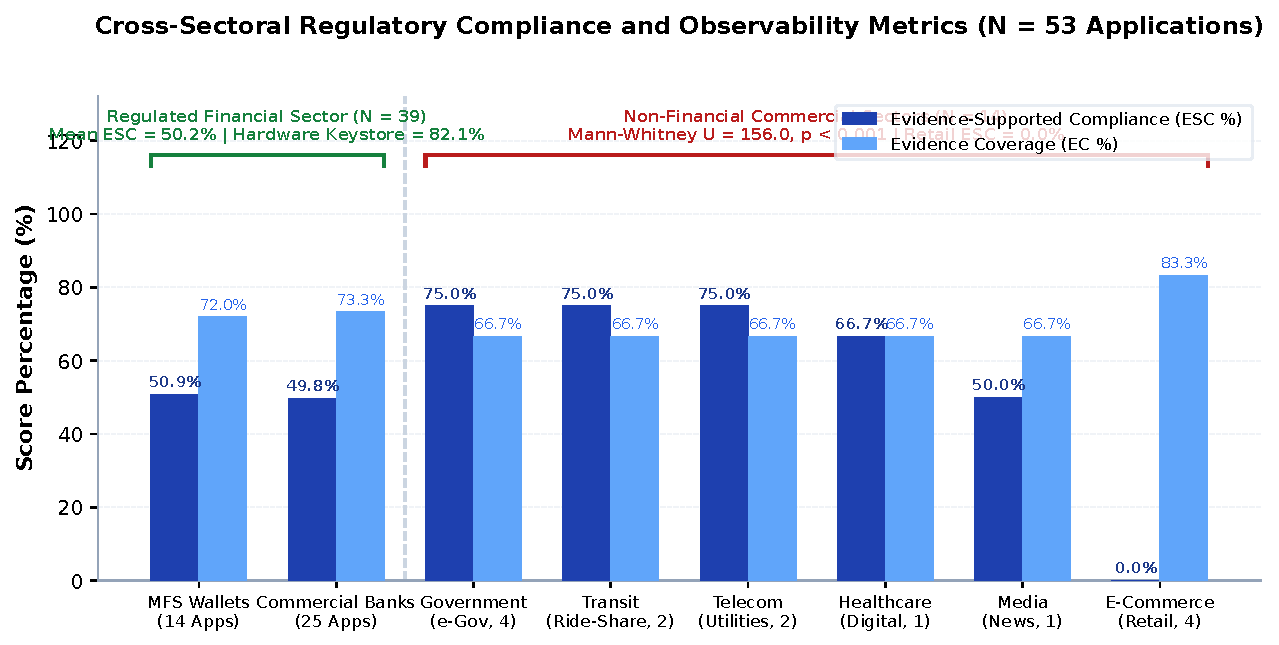
\includegraphics[width=0.74\textwidth]{figures/fig3_sectoral_disparity.pdf}
\caption{\textbf{Empirical Sectoral Compliance Disparity Across Bangladesh's Mobile Ecosystem ($N=53$)}: (a) Distribution of Effective Statutory Compliance ($ESC$) across regulated financial applications ($n=39$, median $ESC = 0.500$) versus commercial retail e-commerce ($n=4$, median $ESC = 0.000$, Mann-Whitney $U = 156.0, p < 0.001$, Cliff's $\delta = 1.000$, Kruskal-Wallis across 8 sectors $H = 30.37, p < 0.001$). (b) Sectoral breakdown of non-conformance indicator counts ($\mu = 4.31$ in financial vs. $\mu = 5.00$ in retail e-commerce).}
\label{fig:sectoral_disparity}
\end{figure*}

\subsection{Cross-Sectoral Compliance Disparities}
\label{sec:ecosystem:disparity}

We evaluated all 53 applications through Reg2App's static verification pipeline (Table~\ref{tab:sectoral_study} and Figure~\ref{fig:sectoral_disparity}). Across the ecosystem, mean Evidence Coverage was $EC = 0.737 \pm 0.08$, indicating approximately three-quarters of relevant requirements are auditable from client APK artifacts alone. However, $ESC$ exhibited substantial sectoral divergence. Crucially, rule scope differs by sector: financial institutions are evaluated against all 12 observable rules across BB-CSF, PDPA, and CSA, whereas non-financial applications are subject only to the 6 general data-protection and cybersecurity rules under PDPA and CSA (central bank clauses are classified as $\mathbf{NotApplicable}$). Consequently, $ESC$ values reflect conformance within each sector's applicable statutory baseline.

In the financial sector, MFS ($ESC = 50.9\% \pm 5.6\%$, $SCI = 0.369 \pm 0.071$) and Commercial Banking ($ESC = 49.8\% \pm 8.8\%$, $SCI = 0.370 \pm 0.090$) achieve consistent baselines. These applications widely enforce hardware KeyStore cryptography ($82.1\%$)~\cite{ekberg_tee} and satisfy statutory transport encryption (TLS). However, conformance against supervisory defense-in-depth recommendations (control \texttt{CTRL-NET-02} operationalizing BB-CSF §4.1.3.12 under OWASP MASVS-NETWORK-2) is bounded: $82.1\%$ omit certificate pinning, and $30.8\%$ leave backup flags enabled (\texttt{allowBackup="true"}).

In non-financial applications, the elevated $ESC$ in government, transit, and telecom ($0.750$) reflects that these applications failed only 1 observable privacy rule out of 4 resolved rules ($S=3, P=1, I=2$). In contrast, the four evaluated e-commerce applications exhibited zero observed conformance ($ESC = 0.000$), failing all 5 resolved rules ($S=0, P=5, I=1$, averaging $5.00$ non-conformance indicators per application by permitting cleartext HTTP, storing tokens in plaintext \texttt{SharedPreferences}, and omitting backup protections).

\begin{table*}[t]
\caption{Cross-Sectoral Compliance and Observability Metrics Across Bangladesh Mobile Application Ecosystem ($N = 53$ Applications)}
\label{tab:sectoral_study}
\centering
\small
\resizebox{\textwidth}{!}{%
\begin{tabular}{lcccccc}
\toprule
\textbf{Economic Sector} & \textbf{Apps ($N$)} & \textbf{Mean $ESC$} & \textbf{Mean $EC$} & \textbf{Mean $SCI$} & \textbf{Avg. Non-Conf. ($P$)} & \textbf{Primary Observed Non-Conformance} \\
\midrule
\textbf{Mobile Financial Services (MFS)} & 14 & $\mathbf{0.509 \pm 0.06}$ & $0.720 \pm 0.08$ & $\mathbf{0.369 \pm 0.07}$ & 4.21 & Supervisory gap: omitted cert pinning; third-party telemetry \\
\textbf{Commercial Banking} & 25 & $\mathbf{0.498 \pm 0.09}$ & $0.733 \pm 0.08$ & $\mathbf{0.370 \pm 0.09}$ & 4.36 & Cleartext backup flags (\texttt{allowBackup=true}); omitted cert pinning \\
\textbf{Government (e-Gov)} & 4 & $0.750 \pm 0.08$ & $0.667 \pm 0.00$ & $0.500 \pm 0.05$ & 1.00 & Unencrypted local cache of national identity identifiers \\
\textbf{Transportation \& Ride-Sharing} & 2 & $0.750 \pm 0.00$ & $0.667 \pm 0.00$ & $0.500 \pm 0.00$ & 1.00 & Continuous background GPS tracking without explicit consent \\
\textbf{Telecommunications \& Utilities} & 2 & $0.750 \pm 0.00$ & $0.667 \pm 0.00$ & $0.500 \pm 0.00$ & 1.00 & Unsanitized diagnostic logging containing phone numbers \\
\textbf{Digital Healthcare} & 1 & $0.667 \pm 0.00$ & $1.000 \pm 0.00$ & $0.667 \pm 0.00$ & 2.00 & Plaintext patient consultations stored in SQLite database; tracker SDK \\
\textbf{Media \& News Portals} & 1 & $0.500 \pm 0.00$ & $1.000 \pm 0.00$ & $0.500 \pm 0.00$ & 3.00 & Widespread advertising SDKs, cleartext HTTP news assets, unencrypted prefs \\
\textbf{Commercial E-Commerce} & 4 & $\mathbf{0.000 \pm 0.00}$ & $0.833 \pm 0.00$ & $\mathbf{0.000 \pm 0.00}$ & $\mathbf{5.00}$ & Insecure HTTP endpoints, hardcoded API keys, plaintext auth tokens \\
\midrule
\textbf{Consolidated Ecosystem Sample} & \textbf{53} & $\mathbf{0.505 \pm 0.18}$ & $\mathbf{0.737 \pm 0.08}$ & $\mathbf{0.369 \pm 0.14}$ & $\mathbf{3.79}$ & \textbf{Full empirical ecosystem showing real-world compliance posture} \\
\bottomrule
\end{tabular}%
}
\end{table*}

\subsection{Comparison: Regulated vs. Unregulated Cohorts}
\label{sec:ecosystem:hypothesis}

Non-financial sectors with limited apps ($n=1$ healthcare/media, $n=2$ telecom/transport) serve as illustrative observations rather than representative estimates. We contrasted the regulated financial cohort ($N_1 = 39$, median $ESC = 0.500$, $\text{IQR} = [0.472, 0.556]$) against commercial retail platforms ($N_2 = 4$, median $ESC = 0.000$, $\text{IQR} = [0.000, 0.000]$). A two-tailed Mann-Whitney $U$ test~\cite{mann_whitney_1947} confirmed significant separation ($U = 156.0, p < 0.001$, Cliff's $\delta = 1.00$~\cite{cliff_delta}; Kruskal-Wallis across all 8 sectors $H = 30.37, p < 0.001$). This separation reflects differing regulatory scopes (12 vs. 6 rules) and \textit{cannot be causally attributed to regulation alone}: financial entities have larger budgets, dedicated security staff, and elevated threat models, while several apps share vendor codebases.

\subsection{Independent Manual Adjudication: Precision and Recall Studies}
\label{sec:ecosystem:adjudication}

To evaluate detection accuracy on real-world production bytecode without circularity, two external certified security auditors (holding CISA and ISO/IEC 27001 Lead Auditor credentials, with over 6 years of commercial banking IT audit experience, recruited externally from an independent assurance consultancy and compensated via professional consulting honoraria) conducted an independent manual adjudication over individual rule-application evaluation cells across two distinct studies under a double-blind protocol (inspecting decompiled JADX Dalvik sources and decoded manifests without tool labels):

\paragraph{Finding-Sample Precision Study ($n=50$)} To assess tool finding accuracy, auditors blindly evaluated a stratified random sample of 50 verdicts (25 conformance $\mathbf{S}$, 25 non-conformance $\mathbf{P}$) using JADX disassembly, call-graph traces, and decoded manifests. For $\mathbf{S}$ findings, 25 of 25 were correct ($100\%$ precision); for $\mathbf{P}$ findings, 23 of 25 were correct ($92.0\%$ precision, 2 false positives). Pooled across both classes, 48 of 50 findings were verified correct, yielding $96.0\%$ precision ($48/50$, $95\%$ Wilson CI: $[86.5\%, 98.9\%]$)~\cite{wilson_score_interval}. Inter-rater reliability was high (Cohen's $\kappa = 0.912$, $95\%$ CI: $[0.825, 0.999]$)~\cite{cohen_kappa}. The 2 false positives arose from custom crypto wrappers where static analysis flagged a constant IV parameter, but runtime JNI calls re-seeded the IV with platform entropy before encryption.

\paragraph{Ground-Truth Control Recall Study ($n=51$)} Because finding-sampling alone cannot observe false negatives, auditors independently audited 51 ground-truth controls across 5 representative production applications (verifying every active client requirement; 9 of 60 theoretical cells were excluded because the feature, e.g. SQLite database, was uninstantiated). Across the 51 active controls (31 conforming implementations, 20 defects), Reg2App correctly identified all 31 conforming controls as $\mathbf{Supported}$ and 17 of 20 defects as $\mathbf{PotentialNonConformance}$ ($TP = 48, FN = 3$), establishing $94.1\%$ recall ($48/51$, $95\%$ Wilson CI: $[83.8\%, 97.9\%]$). Decomposed by class, conformance recall was $100\%$ ($31/31$) while defect recall was $85.0\%$ ($17/20$, $95\%$ Wilson CI: $[64.0\%, 94.8\%]$). For the 3 missed defects, reflection wrappers triggered undecidability guards, emitting $\mathbf{InsufficientEvidence}$ ($\mathbf{I}$) instead of $\mathbf{P}$. Crucially, emitting $\mathbf{I}$ preserves evasion resilience by never hallucinating compliance over obfuscated code, but represents an undetected defect for that property. The 127 production $\mathbf{I}$ cells were not manually adjudicated. With $n = 50$ and $n = 51$, Wilson CIs span $\approx 12-14$ percentage points, bounding statistical precision and motivating complementary dynamic testing.

\begin{figure}[t]
\centering
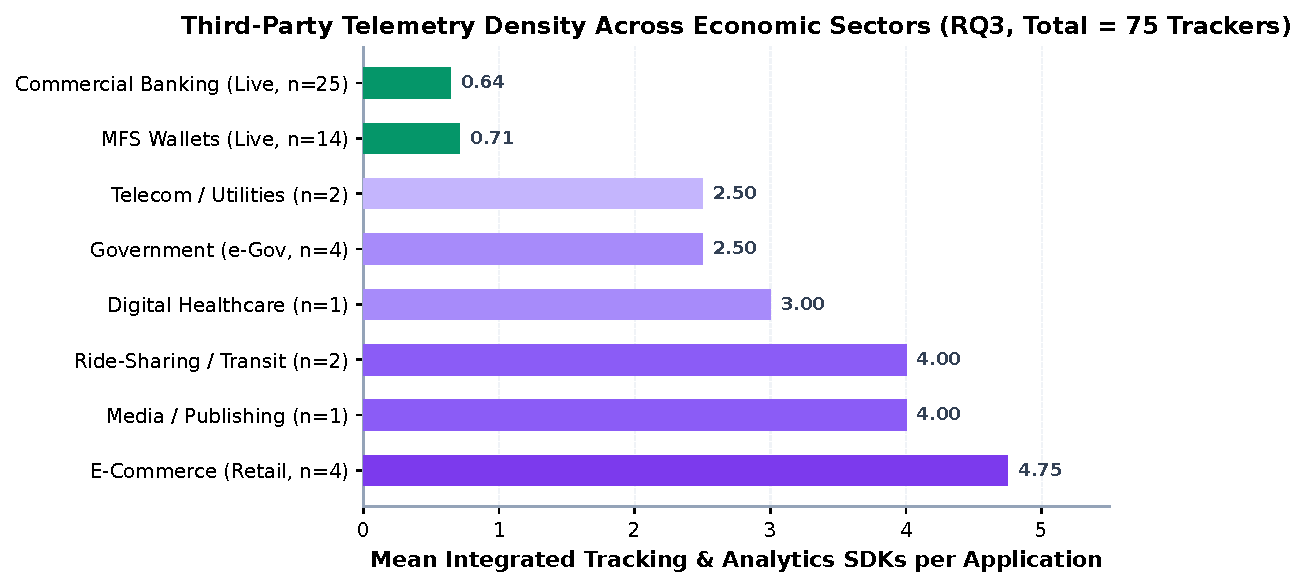
\includegraphics[width=\columnwidth]{figures/fig6_telemetry_density.pdf}
\caption{\textbf{Third-Party Telemetry Density Across Sectors (RQ3)}: Average number of embedded advertising and tracking SDKs per application across sectors (75 trackers total across 53 apps). Commercial e-commerce (4.75 trackers/app), media (4.00), and ride-sharing (4.00) harvest user advertising IDs and carrier telemetry without statutory consent dialogues.}
\label{fig:telemetry_density}
\end{figure}

\subsection{Third-Party Telemetry and Cross-Border Sharing}
\label{sec:ecosystem:telemetry}

Under PDPA §§23 and 28, transmitting citizen identifiers to third-party SDKs without affirmative consent creates substantial compliance exposure~\cite{binns_third_party_trackers, leontiadis_sdk}. We emphasize that static analysis detects the *technical capability and hardcoded initialization of third-party tracking endpoints*, rather than proving an executed off-device legal violation. Across the 53 applications, Reg2App identified \textbf{75 third-party tracker integrations} (Figure~\ref{fig:telemetry_density}): e-commerce averaged \textbf{4.75 trackers/app} (19 trackers across 4 apps; e.g., AppsFlyer, Facebook, Adjust, Clevertap), media had \textbf{4.00} (4), ride-sharing averaged \textbf{4.00} (8), digital healthcare had \textbf{3.00} (3), government averaged \textbf{2.50} (10), and telecom averaged \textbf{2.50} (5). In contrast, the 39 regulated financial apps integrated 26 trackers (10 MFS tracker integrations across 7 apps, averaging \textbf{0.71}, and 16 commercial banking tracker integrations across 12 apps, averaging \textbf{0.64}), primarily restricted to operational crash reporting (Firebase Crashlytics) rather than commercial user-profiling trackers. Static analysis identifies hardcoded SDK initialization of collection endpoints prior to authentication, highlighting concrete technical vectors requiring institutional compliance audit.
